\documentclass[9pt]{beamer}

\usepackage{arabtex}
\usepackage{utf8}

\usepackage{graphicx}

\usetheme{Antibes}
\setbeamertemplate{footline}[frame number]



\begin{document}

\setcode{utf8}

\title{		Why Should We All Learn How to Program?\\ 
			\<
			لماذا علينا جميعا أن نتعلم البرمجة؟
			>
} % !!!! TODO !!!! change color and formatting of "All" and "Program" words
\author{	Ghazi Majdoub\\
			\< 
			غازي المجدوب
			>
}
\date{
			\today\\
			\<
			\today
			>
}

	% ***** Title frame *****
	\begin{frame}
		\titlepage
	\end{frame}
	
	% ***** Table of Content *****
	\section*{
		Overview
		\<
		المحتوى
		>
	}
	\begin{frame}
		\frametitle{
			Overview\\
			\<
			المحتوى
			>
		}
		\tableofcontents
	\end{frame}
	
	% ******************************** THIS PRESENTATION **********************
	% Help people understand:
	% 
	% > What is Programming?
	%
	% > Why programming is important?
	% 1>> Jobs and Professional Success
	% 2>> Power and Control over our lifes
	% 3>> Fight discrimination
	% 4>> Understand our world
	% 5>> Mass Surveillance and Security
	% 6>> Prepare!	
	% 
	% > How to get started and steps to learn programming?
	% *************************************************************************
	
	% ***** What is Programming? *****
	\section{What is Programming?} % !!!! TODO !!!! translate sections titles to arabic (resolve compilation failure)
	\begin{frame}
		\frametitle{
			What is Programming?\\
			\<
			ماهي البرمجة؟
			>
		}
		
		\begin{center}
			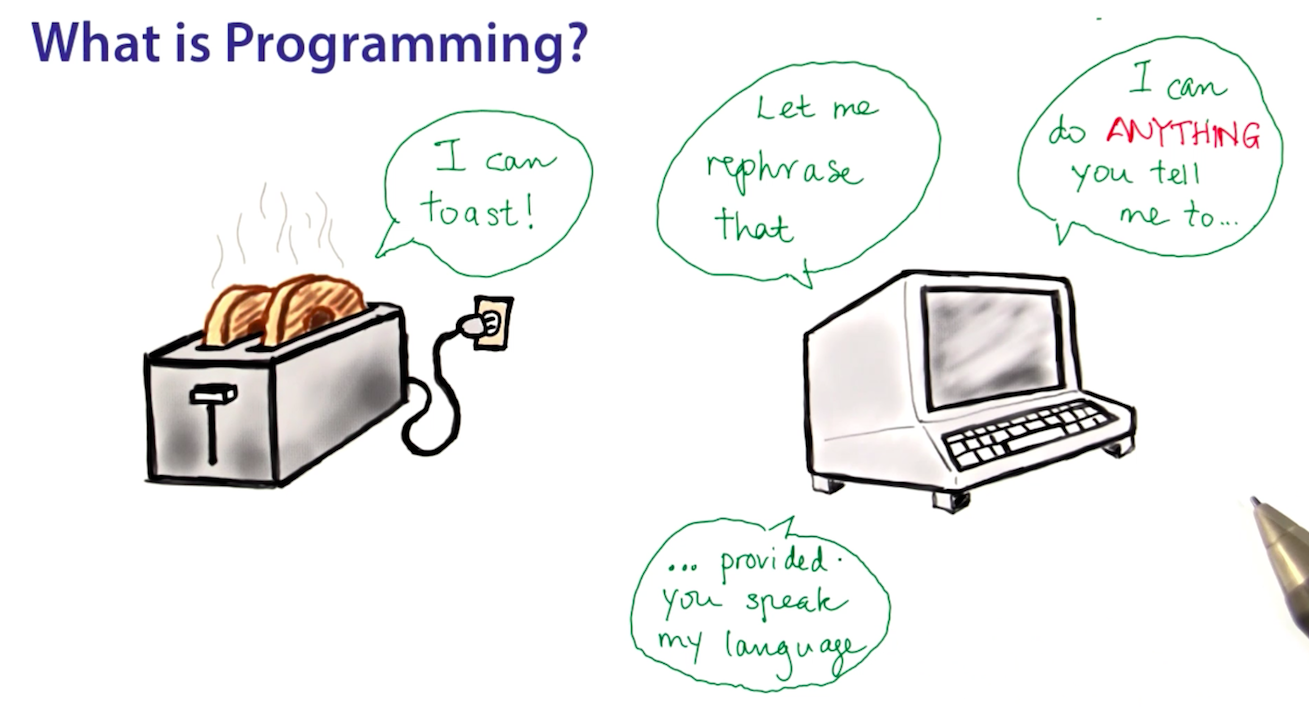
\includegraphics[width=0.6\textwidth]{images/what-is-programming.png}
		\end{center}
		
		\begin{itemize}
			\item	Programming is a lot \textbf{easier} and \textbf{rewarding} than you think!
					\begin{arabtext}
					البرمجة
					\textbf{
						أسهل
					}
					و
					\textbf
					{
						أكبر منفعة
					}
					مما يتصور كثير منكم!
					\end{arabtext}
			\item 	It's not enough anymore to just be able \textbf{to use computers}
					\begin{arabtext}
					لم يعد كافيا فقط تعلّم 
					\textbf{
						استخدام الحاسوب
					}.
					\end{arabtext}
			\item 	It doesn't matter what you do now or plan to do, you \textbf{Need} to Learn how to program.
					\begin{arabtext}
					بغض النظر عن موقعك الآن ومشاريعك المستقبلية،
					\textbf{
						عليك حتما
					}
					تعلّم البرمجة.
					\end{arabtext}
		\end{itemize}
	\end{frame}
	
	% ***** Jobs and Professional success *****
	\section{Jobs and Professional Success}
	\begin{frame}
		\frametitle{
			Jobs and Professional Success\\
			\<
			الوظيفة والنجاح العملي
			>
		}		
	\end{frame}
	
	% ***** Power and Control over our lifes *****
	\section{Power and Control over our lifes}
	\begin{frame}
		\frametitle{
			Power and Control over our lifes\\
			\<
			القوة والتخلص من الهيمنة
			>
		}
	\end{frame}
	
	% ***** Fight discrimination *****
	\section{Fight discrimination}
	\begin{frame}
		\frametitle{
			Fight discrimination\\
			\<
			مقاومة التمييز
			>
		}
	\end{frame}
	
	% ***** Understand our world *****
	\section{Understand our World}
	\begin{frame}
		\frametitle{
			Understand our World\\
			\<
			فهم عالمنا
			>
		}
	\end{frame}
	
	% ***** Mass Surveillance and Security *****
	\section{Mass Surveillance and Security}
	\begin{frame}
		\frametitle{
			Mass Surveillance and Security\\
			\<
			الرقابة الشاملة والأمان الرقمي
			>
		}
	\end{frame}
	
	% ***** Prepare! *****
	\section{Prepare!... For the Second Rise}
	\begin{frame}
		\frametitle{
			"Prepare!"\\
			\<
			وأعدّوا لهم ما استطعتم من قوّة
			>
		}
	\end{frame}
	
	% ***** How to begin? Where? *****
	\section{How to begin? Where?}
	\begin{frame}
		\frametitle{
			How to begin? Where?\\
			\<
			كيف أبدأ ومن أين؟
			>
		}
	\end{frame}
	
\end{document}

